% Template per Elaborato di Laurea
% DISI - Dipartimento di Ingegneria e Scienza dell’Informazione

% formato FRONTE RETRO
\documentclass[epsfig,a4paper,11pt,titlepage,twoside,openany]{book}
\usepackage{epsfig}
\usepackage{plain}
\usepackage{setspace}
\usepackage[paperheight=29.7cm,paperwidth=21cm,outer=1.5cm,inner=2.5cm,top=2cm,bottom=2cm]{geometry} % per definizione layout
\usepackage{titlesec} % per formato custom dei titoli dei capitoli
%\usepackage[italian]{babel}
\usepackage[utf8x]{inputenc} % per Linux (richiede il pacchetto unicode); lettere accentate
\usepackage{listings}
\usepackage{color}
\usepackage{amsmath}
\usepackage{amsfonts}
\usepackage{amssymb}
\usepackage{hyperref} 
\usepackage{xcolor}
\usepackage{color,soul}
\usepackage[bottom]{footmisc}

\usepackage{graphicx} % Required for including images
\usepackage[font=small,labelfont=bf]{caption} 
\definecolor{customLightGray}{RGB}{239, 240, 241}
\DeclareRobustCommand{\code}[1]{{\sethlcolor{customLightGray}\hl{#1}}}
\DeclareRobustCommand{\qt}[1]{{\lq\lq\textit{#1}\rq\rq }}
\DeclareRobustCommand{\u}[0]{{\textunderscore}}

\definecolor{dkgreen}{rgb}{0,0.6,0}
\definecolor{gray}{rgb}{0.5,0.5,0.5}
\definecolor{mauve}{rgb}{0.58,0,0.82}

\lstdefinestyle{CSharpStyle}{
  frame=tb,
  language=[Sharp]C,
  aboveskip=3mm,
  belowskip=3mm,
  showstringspaces=false,
  columns=flexible,
  basicstyle={\small\ttfamily},
  numbers=left,
  numberstyle=\tiny\color{gray},
  keywordstyle=\color{blue},
  commentstyle=\color{dkgreen},
  stringstyle=\color{mauve},
  breaklines=true,
  breakatwhitespace=true,
  tabsize=3
}

\lstdefinestyle{JavaStyle}{
  frame=tb,
  language=Java,
  aboveskip=3mm,
  belowskip=3mm,
  showstringspaces=false,
  columns=flexible,
  basicstyle={\small\ttfamily},
  numbers=left,
  numberstyle=\tiny\color{gray},
  keywordstyle=\color{blue},
  commentstyle=\color{dkgreen},
  stringstyle=\color{mauve},
  breaklines=true,
  breakatwhitespace=true,
  tabsize=3
}

\lstdefinestyle{TeXStyle}{
  frame=tb,
  language=TeX,
  aboveskip=3mm,
  belowskip=3mm,
  showstringspaces=false,
  columns=flexible,
  basicstyle={\small\ttfamily},
  numbers=left,
  numberstyle=\tiny\color{gray},
  keywordstyle=\color{blue},
  commentstyle=\color{dkgreen},
  stringstyle=\color{mauve},
  breaklines=true,
  breakatwhitespace=true,
  tabsize=3
}

\lstdefinestyle{YmlStyle}{
  frame=tb,
  language=TeX,
  aboveskip=3mm,
  belowskip=3mm,
  showstringspaces=false,
  columns=flexible,
  basicstyle={\small\ttfamily},
  numbers=left,
  numberstyle=\tiny\color{gray},
  keywordstyle=\color{blue},
  commentstyle=\color{dkgreen},
  stringstyle=\color{mauve},
  breaklines=true,
  breakatwhitespace=true,
  tabsize=3
}

\lstdefinestyle{QuickstatementsStyle}{
  frame=tb,
  language=TeX,
  aboveskip=3mm,
  belowskip=3mm,
  showstringspaces=false,
  columns=flexible,
  basicstyle={\small\ttfamily},
  numbers=left,
  numberstyle=\tiny\color{gray},
  keywordstyle=\color{blue},
  commentstyle=\color{dkgreen},
  stringstyle=\color{mauve},
  breaklines=true,
  breakatwhitespace=true,
  tabsize=3
}

\lstdefinestyle{SPARQLStyle}{
  frame=tb,
  language=TeX,
  aboveskip=3mm,
  belowskip=3mm,
  showstringspaces=false,
  columns=flexible,
  basicstyle={\small\ttfamily},
  numbers=left,
  numberstyle=\tiny\color{gray},
  keywordstyle=\color{blue},
  commentstyle=\color{dkgreen},
  stringstyle=\color{mauve},
  breaklines=true,
  breakatwhitespace=true,
  tabsize=3
}

\lstdefinestyle{jsonStyle}{
  frame=tb,
  language=TeX,
  aboveskip=3mm,
  belowskip=3mm,
  showstringspaces=false,
  columns=flexible,
  basicstyle={\small\ttfamily},
  numbers=left,
  numberstyle=\tiny\color{gray},
  keywordstyle=\color{blue},
  commentstyle=\color{dkgreen},
  stringstyle=\color{mauve},
  breaklines=true,
  breakatwhitespace=true,
  tabsize=3
}

\singlespacing

\begin{document}
  \pagenumbering{gobble} 
  \pagestyle{plain}

\thispagestyle{empty}

\begin{center}
  \begin{figure}[h!]
    \centerline{
\psfig{file=Sources/logo_unitn_black_center.eps,width=0.6\textwidth}}
  \end{figure}

  \vspace{2 cm} 

  \LARGE{Dipartimento di Ingegneria e Scienza dell’Informazione\\}

  \vspace{1 cm} 
  \Large{Corso di Laurea in\\
    Informatica
  }

  \vspace{2 cm} 
  \Large\textsc{Elaborato finale\\} 
  \vspace{1 cm} 
  \Huge\textsc{Dandelion e Strephit}
  %\Large{\it{Sottotitolo (alcune volte lungo - opzionale)}}


  \vspace{2 cm} 
  \begin{tabular*}{\textwidth}{ c @{\extracolsep{\fill}} c }
  \Large{Supervisore} & \Large{Laureando}\\
  \Large{Alberto Montresor}& \Large{Edoardo Lenzi}\\
  \end{tabular*}

  \vspace{2 cm} 

  \Large{Anno accademico 2018}
  
\end{center}


  \clearpage
  \begin{center}
  {\bf \Huge Ringraziamenti}
\end{center}

\vspace{4cm}

\emph{
Prima di addentrarmi nella descrizione del progetto di tesi voglio ricordare coloro che mi sono stati vicini.
}

\emph{
Ringrazio la mia famiglia per essermi sempre stata accanto ed avermi supportato (e sopportato) in tutti questi anni, permettendomi di studiare fino a laurearmi; ringrazio in particolare mio fratello Massimo e mia sorella Maria Vittoria che più di chiunque altro mi hanno aiutato nello studio.
}

\emph{
Ringrazio i miei zii Chiara e Christian, persone uniche e speciali che da sempre mi sono vicine e mi sostengono. 
}

\emph{
Ringrazio i miei amici, in particolare Michele, dispensatore dei migliori consigli e delle peggiori critiche, senza il quale non avrei nemmeno scelto questa via.
}

\emph{
Ringrazio i miei colleghi di lavoro che mi hanno insegnato moltissimo, facendomi appassionare, di giorno in giorno, sempre più al mio lavoro. 
}

\emph{
Devo, infine, un ringraziamento particolare ad Alberto Montresor, Davide Setti, Alessio Guerrieri, Ugo Scaiella e Marco Fossati che mi hanno seguito ed aiutato moltissimo in questo percorso di tesi.
}

\emph{
A tutti loro va la mia riconoscenza ed i miei più sentiti ringraziamenti.
}

  \clearpage
  \pagestyle{plain} % nessuna intestazione e pie pagina con numero al centro
  % inizio numerazione pagine in numeri arabi
  \mainmatter

  %% Nel conteggio delle facciate (massimo 30) sono incluse: indice, sommario, capitoli
  %% Dal conteggio delle facciate sono escluse: frontespizio, ringraziamenti, allegati

    \tableofcontents % indice
    \clearpage
             
    % gruppo per definizone di successione capitoli senza interruzione di pagina
    \begingroup
      % nessuna interruzione di pagina tra capitoli
      % ridefinizione dei comandi di clear page
      \renewcommand{\cleardoublepage}{} 
      \renewcommand{\clearpage}{} 
      % redefinizione del formato del titolo del capitolo
      % da <Capitolo X> a <X Titolo capitolo>
      
      \titleformat{\chapter}{\normalfont\Huge\bfseries}{\thechapter}{1em}{}
      \titlespacing*{\chapter}{0pt}{0.59in}{0.02in}
      \titlespacing*{\section}{0pt}{0.20in}{0.02in}
      \titlespacing*{\subsection}{0pt}{0.10in}{0.02in}
      
      \chapter*{Sommario} % senza numerazione
\label{sommario}

Il progetto di tesi è il frutto di un tirocinio presso SpazioDati ed una successiva collaborazione al progetto Wikidata StrepHit. La tesi consiste principalmente in tre parti separate, ogniuna delle quali è
legata al servizio online Dandelion (creato da SpazioDati), che verrà brevemente introdotto nelle prossime pagine. 

Il primo capitolo ha lo scopo di introdurre, al lettore, gli applicativi, le tecnologie ed i servizi usati durante il progetto di tesi, descrivendoli sommariamente; 
nei tre capitoli successivi, invece, si entrerà maggiormente nel dettaglio del progetto descrivendo i tre ambiti fondamentali su cui si è focalizzata la tesi.

La prima parte del progetto consiste nell'implementazione di un client in C$\#$, finalizzato allo scopo di creare una libreria di metodi \lq\lq plug$\&$play\rq\rq\ 
per chiamare automaticamente le RESTful-API del servizio Dandelion. 

Durante lo sviluppo il codice è stato regolarmente caricato online, sulla piattaforma GitHub, per agevolare la periodica revisione del codice effettuata dal team di SpazioDati; 
per rendere lo sviluppo più efficiente si è cercato di seguire i principi del TDD (Test Driven Development), affidandosi al servizio di testing automatico Travis 
per validare automaticamente ogni pull-request su GitHub. 

Una volta completata la libreria e l'annessa documentazione è stata compilata la dll e resa pubblica su Nuget; 
pertanto la libreria è ora facilmente integrabile in qualsiasi progetto C$\#$.

La seconda parte del progetto riguarda l'analisi e il test di un algoritmo presente nel backend di Dandelion al fine di ottimizzarlo. 
Il task nasce dalla necessità pratica di ridurre la memoria necessaria alle macchine di produzione di SpazioDati per eseguire l'algoritmo senza subire cali prestazionali.
Partendo dall'implementazione attualmente in uso si sono studiate delle implementazioni alternative per massimizzare la velocità dell'algoritmo e minimizzare 
la memoria occupata dalle strutture dati di appoggio dell'algoritmo. 

L'ultima parte gravita attorno al progetto StrepHit di Wikidata, un progetto nato un anno fa in FBK ed approvato dalla comunity di Wikidata. 
Il progetto nasce per arricchire i database di Wikidata con riferimenti a fonti esterne (tendenzialmente altri siti web) in modo da dare all'utente, fruitore dell'enciclopedia, informazioni sempre più corrette,
validate anche da un sito esterno e non più solo dalla comunity di Wikipedia/Wikidata.

Il progetto è fortemente legato a Dandelion perchè nelle logiche interne dello script di StrepHit si fa largo uso dei servizi offerti da Dandelion per l'analisi testuale delle pagine dei siti esterni.
L'ultima attività consiste nell'implementazione di uno script in python (versione 2.7) utile ad arricchire un dataset di quickstatements aggiungendo riferimenti a proprietà di Wikidata.
Per fare ciò è stato necessario studiare il linguaggio python ed il funzionamento generale di Wikidata per poi realizzare uno script capace di interfacciarsi con l'endpoint SPARQL di Wikidata.
 %massimo 3 pagine 
      \addcontentsline{toc}{chapter}{Sommario} % da aggiungere comunque all'indice
      %%   contesto e motivazioni, breve riassunto del problema affrontato, tecniche utilizzate e/o sviluppate, risultati raggiunti
      \newpage
      
\chapter{Introduzione}
\section{Dandelion}

Dandelion è un servizio online fornito da SpazioDati che mette a disposizione dell'utente servizi di analisi semantica testuale; 
grazie ad esso è possibile, dato un testo, estrarne le entità semantiche principali (\textit{Entity Extraction}), trovare la lingua in cui è stato 
scritto (\textit{Language Detection}), classificarlo secondo modelli definiti dall'utente stesso (\textit{Text Classification}) e analizzarne la semantica 
per capire i sentimenti che l'autore ci vuole trasmettere (\textit{Sentiment Analysis}). 

Dandelion ha anche altre due RESTful-API\footnote{
    \textbf{REST} è un tipo di architettura software per la trasmissione di dati tramite il protocollo HTTP. \href{https://it.wikipedia.org/wiki/Representational_State_Transfer
    }{Fonte} 
} che permettono di confrontare due testi generando un indice di similitudine fra i due (\textit{Text Similarity}) e
un motore di ricerca di entità di Wikipedia (\textit{Wikisearch}), nel caso si voglia trovare il titolo di un contenuto senza conoscerlo a priori.

L'enciclopedia alla base di Dandelion è Wikipedia, anche se a volte fra i due si colloca come mediatore dbpedia\footnote{
    \textbf{DBpedia} è un progetto che ha portato alla creazione di un OKG (Open Knowledge Graph) edificato su informazioni estratte da progetti \href{https://www.wikimedia.org/}{Wikimedia}. \href{https://wiki.dbpedia.org/about}{Fonte}   
}, un progetto italiano per l'estrazione di 
informazioni semi-strutturate da Wikimedia. 

Per poter usare gli end-point di Dandelion basta \href{https://dandelion.eu/accounts/register/}{registrarsi} sul portale dedicato e generare un token che andrà inserito come query parameter nelle chiamate https alle API\footnote{
    La documentazione delle \textbf{API di Dandelion} è disponibile all'indirizzo: \href{https://dandelion.eu/docs/}{https://dandelion.eu/docs/}.
}.

[\textbf{TODO} descrizione dettagliata di Dandelion]
%\subsection{Entity Extraction}
%\subsection{Text Similarity}
%\subsection{Text Classification}
%\subsection{Language Detection}
%\subsection{Sentiment Analysis}
%\subsection{Wikisearch}

\section{GitHub e Travis}
Per il versioning del codice si è scelto di usare il software git\footnote{
    \textbf{Git} è un software open source gratuito per gestire il versioning del codice. \href{https://git-scm.com/}{Sito ufficiale}   
}, appoggiandosi alla piattaforma GitHub per creare repository pubbliche. 

Le repository riguardanti il progetto di tesi sono:

\begin{itemize}
    \item Repository contenente il testo della tesi scritto in \LaTeX\footnote{\url{https://github.com/EdoardoLenzi9/Dandelion.LaTeX}} \\
    \item Repository contenente lo script in Python per il progetto StrepHit\footnote{\url{https://github.com/EdoardoLenzi9/Wikipedia.StrepHit}} \\
    \item Repository contenente il codice Java con le varie implementazioni dell'algoritmo per il calcolo della relatedness (la seconda parte del progetto)\footnote{\url{https://github.com/EdoardoLenzi9/Dandelion.Relatedness}} \\
    \item Repository contenente il codice sorgente del client C$\#$\footnote{\url{https://github.com/EdoardoLenzi9/SpazioDati.Dandelion-eu}}\\
\end{itemize} 

Per quanto riguarda il testing automatico è stata scelta la piattaforma Travis che permette di agganciare una repository GitHub su cui eseguire automaticamente i test 
ad ogni commit. 

Per fare ciò è necessario inserire nella repository un file di configurazione chiamato .travis.yml con i comandi necessari ad eseguire i test. 

Per esempio nel caso del client C$\#$ il file yml contiene le seguenti istruzioni:

\begin{lstlisting}[style=YmlStyle, caption=File configurazione travis.yml per progetti C$\#$]
    language: csharp
    dist: trusty
    mono: none
    dotnet: 2.0.3

    install:
    - dotnet restore

    script:
    - dotnet build
    - dotnet test SpazioDati.Dandelion.Test/SpazioDati.Dandelion.Test.csproj
\end{lstlisting}

Mentre per lo script in Python la sintassi è la seguente:
\begin{lstlisting}[style=YmlStyle, caption=File configurazione travis.yml per progetti Python]
    language: python
    python: 
      - "2.7"
    install:
      - pip install -r requirements.txt
    script:
      - python test.py
\end{lstlisting}

Come si nota dalle righe sopra, basta specificare il linguaggio, la versione ed i comandi\footnote{
    Travis esegue i test in ambiente Linux, quindi i comandi devono essere eseguibili in una bash-shell Linux
}
per installare e lanciare i test.

\section{Docker}
Per la seconda parte del progetto è stato usato Docker\footnote{
    \textbf{Docker} è un progetto open source, cross-platform, che funge da \lq\lq container platform provider\rq\rq\; 
    permette il deployment automatico di applicativi dentro ambienti virtuali chiamati container. \href{https://www.docker.com}{Sito ufficiale}
} per creare un ambiente "chiuso", ad hoc, dove poter testare al meglio gli algoritmi senza doversi preoccupare di fattori esterni che potrebbero falsare 
il risultato del test. 

Docker permette di creare un'immagine a partire da un file di testo chiamato \lq\lq Dockerfile\rq\rq\ il quale contiene tutte le informazioni per eseguire la build dell'immagine; in pratica 
il Dockerfile è una sorta di descrittore dello stato di una macchina virtuale che genera, una volta lanciata la build, una macchina virtuale persistente chiamata immagine. 

Un container è un istanza di un'immagine che diventa quindi non persistente (qualsiasi modifica allo stato della VM verrà perso una volta chiuso il container). 

Una delle caratteristiche più utili di Docker è la semplicità con cui è possibile interfacciare container diversi condividendo aree di memoria sul disco e porte TCP.

L'idea di base per monitorare le prestazioni dell'algoritmo è stata quella di compilare il progetto Java con il tool \href{https://ant.apache.org/}{Ant} ed esportare il file Dandelion.jar; 
è seguita la creazione di un Dockerfile basato sull'immagine \href{https://hub.docker.com/_/openjdk/}{openjdk}, 
scaricata da \href{https://hub.docker.com/}{hub.docker}, contenente un'implementazione open source di Java SE (Java Platform, Standard Edition) a partire dalla versione 7. 

\begin{lstlisting}[style=YmlStyle, caption=Dockerfile]
    FROM openjdk:latest
    COPY . /usr/src/dandelion
    WORKDIR /usr/src/dandelion
    CMD ["java", "-javaagent:./lib/jmx_prometheus_javaagent-0.3.1.jar=8080:./lib/configs.yaml", "-jar", "/usr/src/dandelion/dist/Dandelion.jar"]
\end{lstlisting}

La prima direttiva \code{FROM} specifica l'immagine di base su cui verrà edificata una nuova immagine, le successive due direttive \code{COPY} e \code{WORKDIR} servono rispettivamente a copiare 
tutto il contenuto della cartella corrente dentro l'ambiente virtuale alla path specificata (\textit{/usr/src/dandelion}) e a settare quest'ultima come \textit{working directory} da cui partirà il container docker. 

Infine la direttiva \code{CMD} specifica il comando che verrà eseguito una volta finito il setup dell'ambiente, in questo caso viene eseguito Dandelion.jar con un particolare javaagent chiamato JMX\footnote{
    \textbf{JMX Exporter} è un progetto \href{https://github.com/prometheus/jmx_exporter}{GitHub} open source che fornisce un javaagent capace di esportare ed esporre metrics per il software \href{https://prometheus.io/}{Prometheus}.
};
questo javaagent è un exporter che si occupa di monitorare l'applicativo e di esportare in tempo reale le relative metrics che vengono esposte in un server locale su una porta a scelta (8080 in questo caso).

Per evitare di effettuare una build del Dockerfile ogni volta che modifichiamo il codice sorgente Java è possibile mappare la cartella corrente con la working directory dell'immagine tramite l'opzione \code{-v}
che crea un volume condiviso; tramite l'opzione \code{-p} invece è possibile mappare una porta tcp interna al docker su una esterna.

\begin{lstlisting}[style=YmlStyle, caption=Run Docker]
    docker run -it -p 8080:8080 -v <current-dir>.:<docker-working-dir> \
    --name dandelion-volume dandelion-container
\end{lstlisting}

\section{Prometheus e Grafana}
Parallelamente al primo container vengono istanziate altre due immagini, scaricate da \href{https://hub.docker.com/}{hub.docker}, chiamate \href{https://hub.docker.com/r/prom/prometheus/}{prom/prometheus} 
e \href{https://hub.docker.com/r/grafana/grafana/}{grafana/grafana} le quali permettono di filtrare le metrics generate dall'exporter e di visualizzarle direttamente su dei grafici. 

\subsection{Prometheus}
\href{https://prometheus.io/}{Prometheus} è un applicativo open source rilasciato sotto Apache 2 License su GitHub, permette di salvare in memoria e/o sul disco le metrics raccolte da un exporter e mette a disposizione 
un linguaggio di query che permette di filtrare le metrics a piacimento. 

È anche possibile rappresentare i risultati delle query direttamente su dei grafici statici tuttavia per questo aspetto si è scelto di usare Grafana.

\subsection{Grafana}
\href{https://grafana.com/}{Grafana} è anch'essa un software open source volto alla creazione di dashboard dinamiche tipicamente consistenti in grafici e widget di monitoraggio di vario tipo, funzionalmente molto completi 
e gradevoli sotto il profilo estetico. 

Grafana è nativamente predisposta per integrarsi con Prometheus, basta indicare la porta tcp su cui è settato Prometheus e la query che si desidera visualizzare.   

\section{Wikidata e StrepHit}
Wikidata è un progetto gratuito e open source legato a Wikipedia che mette a disposizione dell'utente un knowledge base accessibile sia dal portale wikidata.org che tramite un end-point SPARQL.

I dati presenti nel knowledge base sono dati strutturati secondo le logiche del semantic web e adottano, quindi, il framework RDF (Resource Description Framework) proposto da W3C. 

Questo servizio rende possibile l'interazione con il knowledge base di Wikidata direttamente tramite query veicolate da chiamate http ad un end-point SPARQL ed è facilmente integrabile 
con qualsiasi altro knowledge base di terze parti che segua gli stessi schemi e modelli RDF.

\href{https://www.mediawiki.org/wiki/StrepHit}{StrepHit} è un progetto nato l'anno scorso, seguito da un team in FBK, coordinato da Marco Fossati; il progetto prevedeva la creazione di un applicativo scritto prevalentemente 
in python capace di analizzare testi e tradurli in Wikidata statements (o QuickStatements).  

\href{https://www.mediawiki.org/wiki/StrepHit}{QuickStatemens} è un tool scritto da Magnus Manske che definisce un linguaggio volto a descrivere/modificare elementi Wikidata. Questo linguaggio è ormai diventato uno standard 
per quanto riguarda Wikidata tant'è che la nomenclatura degli elementi del knowledge base seguono gli standard dettati da Quickstatements.

\subsection{SPARQL}
\href{https://www.w3.org/TR/sparql11-query/}{SPARQL} è il linguaggio di query definito da W3C per RDF. Le query sono molto affini al SQL, infatti ne condividono molte key-word, la differenza sta nel fatto che i dati ora 
seguono i modelli RDF pertanto avranno sempre un item, una property e un value.

Wikidata mette a disposizione \href{https://query.wikidata.org/}{un'interfaccia} che permette di lanciare manualmente query SPARQL sul knowledge base
e un \href{https://query.wikidata.org/bigdata/namespace/wdq/sparql?query={SPARQL}}{end-point} per contattare lo stesso servizio con chiamate http. 

      \newpage
      \addcontentsline{toc}{chapter}{Client C$\#$}

\chapter{Client C$\#$}
%%%%%%%%%%%%%%%%%%%%%%%%%%%%%%%%%%%%%%%%%%%%%%%%%%%%%%%%%%%%%%%%%%%%%%%%%%%%%%%%%%%%%%%%%%%%%%%%%%%%%%%%%%%%%%%%%%%%%%%%
\section{Struttura Generale}

Per l'implementazione si è cercato di seguire le best practices, dettate dalle linee guida Microsoft, per la stesura del codice.
Sono stati adottati, come pattern di programmazione, dependency injection\footnote{
    \textbf{Dependency injection}~\cite{dependency-injection} è un pattern di programmazione che prevede la risoluzione automatica delle dipendenze delle classi 
    (può essere usata direttamente nel costruttore o nei metodi) tramite un injector (inversion of control).

        \textbf{Inversion of control}~\cite{inversion-of-control} è una macro categoria di pattern (ingloba al suo interno anche dependency injection)
        secondo cui, in certi punti del codice, si riceve il controllo di determinate funzioni di un framework.
}, MVC\footnote{
    \textbf{Model-View-Controller (MVC)}~\cite{mvc} è un pattern di programmazione che prevede un architettura multi-tier con una netta divisione fra modelli, 
    business logic e interfaccia utente (in questo caso praticamente assente).
} (per quanto possibile) e TDD, appoggiandosi a librerie esterne Nuget\footnote{
    \textbf{Nuget}~\cite{nuget} è un package manager per .NET.
} quali \code{Newtonsoft.Json}~\cite{newtonsoft-json} e \code{SimpleInjector}~\cite{simple-injector}. 

Si è cercato di adottare il più possibile i dettami della programmazione asincrona e di rendere il client thread-safe.

Il file solution\footnote{
    \textbf{Solution} è un file, con estensione \code{.sln}, che serve per raggruppare più progetti C$\#$ in un unico macro contenitore.  
} è stato partizionato in vari progetti; il progetto \code{Business} contiene la business-logic 
(comprendente servizi, metodi estensione, l'implementazione del client e un wrapper del \code{Container} di \code{SimpleInjector}) e utilizza i modelli di \code{Domain}.

In \code{Test} sono contenute le classi di testing e le fixture \code{XUnit}\footnote{
    \textbf{XUnit}~\cite{xunit-repo} è una libreria Nuget~\cite{xunit} che mette a disposizione un tool per eseguire unit test.     
}, mentre in \code{Documentation} sono presenti i file generati dal tool Wyam\footnote{
    \textbf{Wyam}~\cite{wyam} è un tool che permette l'esportazione della documentazione del codice C$\#$ 
    (sottoforma di tag xml~\cite{code-doc}) in pagine html.
} per la documentazione.

%%%%%%%%%%%%%%%%%%%%%%%%%%%%%%%%%%%%%%%%%%%%%%%%%%%%%%%%%%%%%%%%%%%%%%%%%%%%%%%%%%%%%%%%%%%%%%%%%%%%%%%%%%%%%%%%%%%%%%%%
\section{Il Client}

Dalla documentazione ufficiale~\cite{dandelion-doc} delle API di Dandelion si evince che ogni endpoint richiede uno o più testi da analizzare ed una serie di parametri, 
alcuni obbligatori ed altri opzionali; 
pertanto sono stati creati dei modelli, coerenti con tali definizioni, che, passati in argomento a dei servizi, ritornano i DTO delle risposte degli endpoint di Dandelion.

Ogni servizio controlla che i parametri inseriti dall'utente rispettino i vincoli definiti nella documentazione e costruisce, tramite i metodi \code{ContentBuilder()} e  
\code{UriBuilder()}, un dizionario di parametri e l'URI che identifica l'endpoint. 

Infine il servizio chiama il metodo generico \code{CallApiAsync()}, passandogli il content, la URI ed il metodo HTTP; 
nel metodo di chiamata si è scelto di gestire separatamente i metodi HTTP GET e DELETE dato che essi non permettono il passaggio parametri nel body 
della chiamata. Pertanto è stato necessario inviare il content come query parameter facendone il percent-encoding.

Dandelion ammette sia chiamate GET che POST ai servizi, tuttavia nel caso del metodo GET non è garantito il corretto 
funzionamento del servizio per testi che superano i 2000 caratteri; pertanto nel caso in cui l'utente non specifichi il metodo HTTP, di default verrà
usato il metodo POST.

Se la chiamata è andata a buon fine il JSON di ritorno viene mappato in un DTO specifico, a seconda del servizio scelto, e restituito direttamente all'utente.

\begin{lstlisting}[style=CSharpStyle, caption=Metodo generico del client per le chiamate HTTP]
public Task<T> CallApiAsync<T>(string uri, List<KeyValuePair<string, string>> content, HttpMethod method = null)
{
    var result = new HttpResponseMessage();
    if (method == null)
    {
        method = HttpMethod.Post;
    }

    if (_client.BaseAddress == null)
    {
        _client.BaseAddress = new Uri(Localizations.BaseUrl);
    }

    return Task.Run(async () =>
    {
        if (method == HttpMethod.Get)
        {
            string query;
            using (var encodedContent = new FormUrlEncodedContent(content))
            {
                query = encodedContent.ReadAsStringAsync().Result;
            }
            result = await _client.GetAsync($"{uri}/?{query}");
        }
        else if (method == HttpMethod.Delete)
        {
            string query;
            using (var encodedContent = new FormUrlEncodedContent(content))
            {
                query = encodedContent.ReadAsStringAsync().Result;
            }
            result = await _client.DeleteAsync($"{uri}/?{query}");
        }
        else
        {
            var httpContent = new HttpRequestMessage(method, uri);
            if (content != null)
            {
                httpContent.Content = new FormUrlEncodedContent(content.ToArray());
            }
            result = await _client.SendAsync(httpContent);
        }
        string resultContent = await result.Content.ReadAsStringAsync();
        if (result.StatusCode == System.Net.HttpStatusCode.RequestUriTooLong)
        {
            throw new ArgumentException(ErrorMessages.UriTooLong);
        }
        if (!result.IsSuccessStatusCode)
        {
            throw new Exception(resultContent); 
        }
        return JsonConvert.DeserializeObject<T>(resultContent);
    });
}
\end{lstlisting}

\section{Testing}
La maggior parte dei servizi è stata testata tramite il tool XUnit; principalmente sono stati eseguiti test di validazione, data la natura della libreria, appoggiandosi 
ad una fixture comune a tutti i test per l'inizializzazione dei servizi.

É stato usato fin da subito il servizio online di testing automatico Travis, tramite il quale è stato possibile validare ogni rilascio facendo 
partire automaticamente i test con l'evento di push di Git. 

\section{Documentazione}
Infine le classi e i metodi più rilevanti sono stati commentati tramite i tag XML specificati nella documentazione Microsoft e la documentazione in formato 
HTML è stata generata automaticamente tramite il tool Wyam.

\section{Nuget}
La \code{.dll} generata dalla compilazione della libreria è stata infine documentata sotto il profilo delle dipendenze, generando il file \code{.nuspec}, ed inclusa nel file 
\code{.nupkg} tramite l'apposito tool fornito da Nuget. Il tutto è stato caricato sul portale online Nuget ed è ora possibile includerlo in un progetto tramite il comando cli:

\begin{lstlisting}[style=TexStyle, caption=Comando cli per includere il client in un progetto]    
$ dotnet add package SpazioDati.Dandelion
\end{lstlisting}

\section{Demo}
Per provare il client basta creare un programma cli di test:

\begin{lstlisting}[style=TexStyle, caption=Creazione di un progetto demo]    
    $ mkdir Demo && cd Demo
    $ dotnet new console
    $ dotnet add package SpazioDati.Dandelion
    $ dotnet restore
\end{lstlisting}

Nel file \code{Program.cs} sostituire il seguente codice e lanciare il programma:
\begin{lstlisting}[style=CSharpStyle, caption=Codice per chiamare Entity Extraction API]    
    using System;
    using System.Net.Http;
    using Newtonsoft.Json;
    using SpazioDati.Dandelion.Business;
    using SpazioDati.Dandelion.Domain.Models;
    
    namespace Demo
    {
        class Program
        {
            static void Main(string[] args)
            {
                var token = "<your-token>";
                var text = "the quick brown fox jumps over the lazy dog";
                var entities = DandelionUtils.GetEntitiesAsync(new EntityExtractionParameters{Token = token, Text = text, HttpMethod = HttpMethod.Post});
                Console.WriteLine(JsonConvert.SerializeObject(entities));
            }
        }
    }
\end{lstlisting}   

\begin{lstlisting}[style=TexStyle, caption=Compilare e lanciare il programma]    
    $ dotnet run
\end{lstlisting}

      \newpage
      \chapter{Calcolo della Relatedness}

La seconda parte del progetto riguarda l'analisi di due metodi critici (\code{readDump()} e \code{rel(int a, int b)}) che servono a 
calcolare, dati gli identificativi di due entità semantiche, il loro valore di correlazione (relatedness). 

Per fare ciò si ha a disposizione un dump dove sono salvati tutti i valori di correlazione (sopra una certa soglia minima) per ogni coppia di entità. 

Il metodo \code{readDump()} serve a caricare in memoria i valori del dump 
sottoforma di \lq\lq matrice\rq\rq\ mentre il metodo \code{rel(int a, int b)} serve a fare una ricerca nella struttura dati per poi ritornare il valore di 
correlazione fra le entità con identificativi \code{a} e \code{b}.

Questa scelta implementativa, attualmente adottata, è sicuramente molto efficiente in termini di prestazioni ma sicuramente molto onerosa in termini di memoria; 
pertanto il fine dell'analisi sarebbe quello di studiare/testare implementazioni alternative per ottimizzare le prestazioni e/o diminuire lo spreco di memoria.  

%%%%%%%%%%%%%%%%%%%%%%%%%%%%%%%%%%%%%%%%%%%%%%%%%%%%%%%%%%%%%%%%%%%%%%%%%%%%%%%%%%%%%%%%%%%%%%%%%%%%%%%%%%%%%%%%%%%%%%%%
\section{Implementazione Iniziale}

%%%%%%%%%%%%%%%%%%%%%%%%%%%%%%%%%%%%%%%%%%%%%%%%%%%%%%%%%%%%%%%%%%%%%%%%%%%%%%%%%%%%%%%%%%%%%%%%%%%%%%%%%%%%%%%%%%%%%%%%
\subsection{Il Dump}
\begin{lstlisting}[style=TeXStyle, caption=Estratto del dump]
53676192
4922289
0.01
2
1.0
53676158 7 null
53676164 5 NnAwQT/ZvTVJ05MeSfcdI0rMrg1LBmUH
53676016 13 RDsFRUkyASRLFf3T
53675811 16 null
...
\end{lstlisting}

Leggendo le prime righe di un dump si nota che le prime cinque righe sono valori di inizializzazione mentre dalla sesta righa in poi troviamo le righe della matrice.
Il primo numero intero, denominato \textit{max$\_$id}, indica il limite massimo che gli id delle entità possono assumere; 
dato che gli id delle entità non sono necessariamente sequenziali 
(fra due di essi potrei avere dei \lq\lq buchi\rq\rq, degli intervalli in cui gli identificativi non sono associati ad alcuna entità) 
esiste una funzione \textit{map} che mappa (\lq\lq compatta\rq\rq) gli id delle entità su altri id univoci e sequenziali. 

Il secondo intero, denominato \textit{nodesSize} è il valore massimo che la funzione \textit{map} può assumere (limita il codominio della funzione).

\begin{equation}\begin{split}
    map():\ \mathbb{N} & \rightarrow \mathbb{N}\\
            [0,max\_id] & \rightarrow [0, nodeSize], max\_id \geq nodeSize\\
\end{split}\end{equation}

Continuando a leggere il dump troviamo la relatedness minima considerata \textit{minRel} (sotto la quale i valori di correlazione non vengono salvati) 
e altri valori di configurazione quali \textit{minIntersection} e \textit{threshold} che tuttavia non ci interessano particolarmente.

La funzione map in un certo senso mappa \lq\lq al contrario\rq\rq\ gli id; infatti l'id massimo verrà mappato su 0, il penultimo id verrà mappato su 1 e così via.
Nel caso del dump in questione abbiamo:

\begin{lstlisting}[style=TeXStyle, caption=Esempio di funzione map e postingList]
MaxId = 53676192
NodeSize = 4922289

   ID		        MAP(ID)    POSTINGLIST
...
53676158    ->      7           null
53676159    ->      6           FW/I...
53676164    ->      5           NnAw...
53676174    ->      4           null
53676176    ->      3           null
53676177    ->      2           null
53676180    ->      1           null
53676190    ->      0           null
\end{lstlisting}

Gli id presenti nel dump non sono ordinati ma le \textit{postingList} ad essi associate lo sono.

Dalla sesta riga del dump in poi inizia la definizione della matrice, ogni riga è composta da tre valori separati da uno spazio. 
Ad esempio se consideriamo la riga:
\begin{lstlisting}[style=TeXStyle, caption=Riga del dump]
53676164 5 NnAwQT/ZvTVJ05MeSfcdI0rMrg1LBmUH
\end{lstlisting}

Il primo valore $a = 53676164$ è l'id di un entità, il secondo valore $b = 5 = map(a)$ è il risultato della funzione map, 
infine il terzo valore $c = NnAwQT/ZvTVJ05MeSfcdI0rMrg1LBmUH$ è una stringa di dimensione variabile oppure \textit{null};
quest'ultima stringa, denominata \textit{postingList}, è la codifica in \textit{Base64} di un array di byte che rappresenta un dizionario chiave valore. 

\begin{center}
    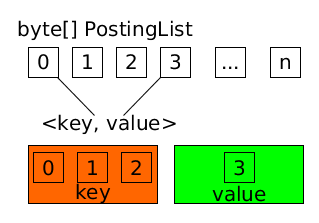
\includegraphics[scale=0.55]{Sources/Img/c02_01.png}
    \captionof{figure}{Encoding del dizionario nella postingList}
\end{center}

In pratica una tupla $<chiave,\ valore>$ è codificata sull'array da una sequenza di quattro byte; quindi partizionando l'array in gruppi da 4 byte 
ottengo, per ogni gruppo, la chiave (è un id \lq\lq mappato\rq\rq ) codificata sui primi tre byte ed il valore (la relatedness) definito sul quarto byte (il byte più a destra).

Questa codifica, pertanto, permette di gestire set di entità con id \lq\lq mappato\rq\rq\ massimo $2^{3 \cdot 8} \simeq 1,7 \cdot 10^7$ ed una scala di valori 
di correlazione appartenenti all'intervallo $[0,\ 255]$.

Bisogna precisare che l'array di byte, denominato \textit{postingList}, è ordinato per valore crescente delle chiavi e, dato che rel(a, b) = rel(b, a),
si è deciso di salvare una sola volta il valore di correlazione imponendo la relazione: $a > b$.

%%%%%%%%%%%%%%%%%%%%%%%%%%%%%%%%%%%%%%%%%%%%%%%%%%%%%%%%%%%%%%%%%%%%%%%%%%%%%%%%%%%%%%%%%%%%%%%%%%%%%%%%%%%%%%%%%%%%%%%%
\subsubsection{Esempio}
Nell'ipotesi in cui abbia una riga nel dump costituita dalla tupla $(a,\ b,\ c)$ e volessi trovare $relatedness(a, d)$ con $map(a) > map(d)$. 

Devo cercare nella \textit{postingList c}, un gruppo di quattro byte in cui i primi tre byte corrispondano a \textit{map(d)} ed il quarto byte sarà il valore di correlazione voluto. 

Ovviamente è possibile che \textit{c} sia \textit{null} (l'entità con id \textit{a} non ha nessuna correlazione con entità i cui id \lq\lq mappati\rq\rq\ siano inferiori a \textit{b}) oppure 
che nella posting non sia presente nessuna chiave corrispondente a \textit{map(d)}, in questi casi $relatedness(a,d) = 0$. 

%%%%%%%%%%%%%%%%%%%%%%%%%%%%%%%%%%%%%%%%%%%%%%%%%%%%%%%%%%%%%%%%%%%%%%%%%%%%%%%%%%%%%%%%%%%%%%%%%%%%%%%%%%%%%%%%%%%%%%%%
\subsection{Il Codice Nativo}

\begin{lstlisting}[style=JavaStyle, caption=Implentazione nativa]
// STRUTTURA DATI
public class RelatednessMatrix {
    public int[] map;
    public byte[][] matrix;
    public float configuredMinRel;
    public int configuredMinIntersection;
    public float threshold;
    public static int EL_SIZE = 4;
}

// CODICE UTILIZZO
public float rel(int a, int b){
    if(a==b) return 1f;

    int nodeA = data.map[a];
    int nodeB = data.map[b];
    if (nodeA < 0 || nodeB < 0) return 0f;

    int key = a>b ? nodeB : nodeA;
    byte[] array = a>b ? data.matrix[nodeA] : data.matrix[nodeB];

    if (array == null) return 0f;

    int start = 0;
    int end = array.length - RelatednessMatrix.EL_SIZE;
    int pos = -1;
    while(pos == -1 && start <= end)
    {
        int idx = ((start+end)/RelatednessMatrix.EL_SIZE)/2;
        int idx_value = ((array[idx*RelatednessMatrix.EL_SIZE] & 0xFF) << 16)
                    + ((array[idx*RelatednessMatrix.EL_SIZE+1] & 0xFF) << 8)
                    + ( array[idx*RelatednessMatrix.EL_SIZE+2] & 0xFF);

        if(idx_value == key) pos = idx;
        else{
            if(key > idx_value)
                start = (idx + 1) * RelatednessMatrix.EL_SIZE;
            else
                end = (idx - 1) * RelatednessMatrix.EL_SIZE;
        }
    }

    if(pos == -1) return 0f;
    else
    {
        byte by = array[pos * RelatednessMatrix.EL_SIZE + 3];
        int byint = by + 128;
        float byteRel = byint / 255f;
        return data.configuredMinRel + byteRel * (1 - data.configuredMinRel);
    }
}

// CODICE LETTURA
public String END_OF_FILE = "" + '\0';

public RelatednessMatrix readDump() throws Exception {
    URL url = getClass().getResource("dump.txt");
    File file = new File(url.getPath());
    BufferedReader fbr = new BufferedReader(new FileReader(file));
    String line = new String();

    try {   
        int max_id = Integer.parseInt(fbr.readLine().trim()); // Trims all leading and trailing whitespace from this string         
        int nodesSize = Integer.parseInt(fbr.readLine().trim());
        float minRel = Float.parseFloat(fbr.readLine().trim());
        int minIntersection = Integer.parseInt(fbr.readLine().trim());
        float threshold = Float.parseFloat(fbr.readLine().trim());         

        RelatednessMatrix data = new RelatednessMatrix();
        data.map = new int[max_id + 1];
        data.matrix = new byte[nodesSize][];
        data.configuredMinRel = minRel;
        data.configuredMinIntersection = minIntersection;
        data.threshold = threshold;

        int idx = 0;

        while ((line = fbr.readLine()) != null) {
            if (line.trim().equals(END_OF_FILE.trim())) {
                break;
            }
            System.out.println(line);
            String[] splittedLine = line.split("\\s+"); // split(" ")
            if (splittedLine.length != 3) {
                throw new Exception("Wrong format relatedness file for the line: " + line);
            }

            int wid = Integer.parseInt(splittedLine[0]);
            int node = Integer.parseInt(splittedLine[1]);
            data.map[wid] = node;

            if (splittedLine[2].equals("null")) {
                data.matrix[node] = null;
            } else {
                byte[] a = Base64.getDecoder().decode(splittedLine[2].toString()); 
                data.matrix[node] = Base64.getDecoder().decode(splittedLine[2].toString());
            }
            idx++;
        }
        
        if (idx != nodesSize) {
            throw new Exception("Wrong format relatedness file the number of line do not match with size of matrix");
        }
        
        return data;
    } catch (Exception e) {
        System.out.println(e.getMessage());
        return null;
    }
}
\end{lstlisting}

Il metodo \code{readDump()} legge riga per riga il dump e restituisce un'istanza di RelatednessMatrix valorizzata. 
La funzione map viene salvata in un array di interi (\code{data.map}) mentre la matrice con le correlazioni viene salvata in un 
array bidimensionale di byte (\code{data.matrix}).

Il metodo \code{rel(int a, int b)} invece calcola la funzione \code{map} sugli id \code{a} e \code{b} dopodichè fa una binary search sulla postingList 
ottenuta da matrix[map(a)] (assumendo $map(a) > map(b)$). Infine se la ricerca binaria ha successo il valore di relatedness ottenuto va riscalato su una scala di valori 
$[0, 255]$, convertito in float e riscalato nuovamente in base al valore di relatedness minima considerata (per escludere i valori al di sotto della relatedness minima,
che non verranno mai usati).  

\begin{lstlisting}[style=JavaStyle, caption=Conversione della relatedness da byte a float]
byte by = array[pos * RelatednessMatrix.EL_SIZE + 3]; //considero il quarto byte 
int byint = by + 128;   //scalo di 128 valori per ottenere una relatedness in [0, 255]

//cast in float, escludendo i valori sotto la relatedness minima (configuredMinRel)
float byteRel = byint / 255f; 
return data.configuredMinRel + byteRel * (1 - data.configuredMinRel);
\end{lstlisting}

%%%%%%%%%%%%%%%%%%%%%%%%%%%%%%%%%%%%%%%%%%%%%%%%%%%%%%%%%%%%%%%%%%%%%%%%%%%%%%%%%%%%%%%%%%%%%%%%%%%%%%%%%%%%%%%%%%%%%%%%
\subsection{Osservazioni}
Considerato che il metodo \code{readDump()} viene chiamato una sola volta per allocare in memoria la struttura dati nel server, 
non ci sono particolari vincoli temporali per la sua esecuzione; per quanto riguarda il calcolo della relatedness invece 
l'algoritmo dev'essere il più performane possibile.

Il codice nativo per il calcolo della relatedness costa $O(lg_2(n))$ (con $n=nodeSize$) per la ricerca binaria e O(1) per quanto riguarda le 
istruzioni precedenti e successive a quest'ultima.

Tolto un piccolo refact del codice che portebbe ad evitare tre moltiplicazione per ciclo nella binary search (non è necessario dividere e poi moltiplicare per 
RelatednessMatrix.EL$\_$SIZE), non sembra si possono migliorare di molto le prestazioni dell'algoritmo senza cambiare struttura dati.

Una via percorribile per non \lq\lq pagare\rq\rq\ $O(lg_2(n))$ per la binary search potrebbe essere quella di allocare direttamente in memoria la matrice 
completa (in questo caso avrei un algoritmo di tempo costante O(1)). Questa soluzione però andrebbe a peggiorare drasticamente lo spreco di memoria.
Infatti nell'implementazione attuale la matrice ha dimensione massima $nodeSize \otimes nodeSize$ ma le righe hanno dimensione variabile e 
non occupano quindi sempre $(nodeSize -1) \cdot 4\ Byte$.

%%%%%%%%%%%%%%%%%%%%%%%%%%%%%%%%%%%%%%%%%%%%%%%%%%%%%%%%%%%%%%%%%%%%%%%%%%%%%%%%%%%%%%%%%%%%%%%%%%%%%%%%%%%%%%%%%%%%%%%%
\subsubsection{Stima della Memoria Allocata}
Se consideriamo le prime righe del dump in questione possiamo stimare che mediamente il $57\%$ degli id hanno postingList vuota (null) ed il restante $43\%$ ha un numero 
medio di relatedness per id pari allo $0,000101\%$ di nodeSize.

L'implementazione attuale alloca in memoria per l'array di interi map circa:
\begin{center}
\begin{equation}\begin{split} 
    nodeSize \cdot 4\ Byte & = 4^2 \cdot 10^6 Byte = 16 MB \\
\end{split}\end{equation}
(arrotondando e senza tenere conto di fattori secondari come i 32 byte occupati da overhead e puntatore).
\end{center}
Per la matrice invece possiamo assumere che, su una macchina a 64 bit, avrò il $57\%$ di righe a null ($0.57 \cdot 4\cdot 10^6 \cdot 8\ Byte = 18\ MB$) ed il 
restante $43\%$ di righe con mediamente 404 valori di relatedness codificati su 4 Byte ($0.43 \cdot 4 \cdot 10^6 \cdot 404 \cdot 4\ Byte = 2.8\ GB$). 

Quindi in totale potremmo stimare che solo questo dump occupa quasi 3 GB (notare che esiste un dump per ogni lingua supportata da Dandelion e che questo è uno 
dei dump più piccoli).

%%%%%%%%%%%%%%%%%%%%%%%%%%%%%%%%%%%%%%%%%%%%%%%%%%%%%%%%%%%%%%%%%%%%%%%%%%%%%%%%%%%%%%%%%%%%%%%%%%%%%%%%%%%%%%%%%%%%%%%%
\subsubsection{Stima della Matrice Completa}
Se allocassimo in memoria una matrice di Byte completa, di dimensioni $nodeSize \otimes nodeSize$, essa occuperebbe $(4 \cdot 10^6)^2 = 1.6 \cdot 10^{13}\ Byte = 16\ TB$.
Pur considerando che esistono strutture dati particolarmente ottimizzate per gestire array di grandi dimensioni con pochi valori al loro interno (teniamo presente che
più della metà dei valori nella matrice non saranno valorizzati), come SparseArray e SuperArrayList, bisogna tener presente che spesso tali strutture dati 
si basano su liste; in questo caso però difficilmente si otterrebbero prestazioni migliori di quelle dell'implementazione attuale dato che il tempo di lookup 
sarebbe sempre $O(lg_2(noseSize))$. 

In conclusione, a meno di uno spreco di memoria ulteriore, difficilmente otterremo buoni risultati mantenendo come struttura dati di riferimento la matrice. 

%%%%%%%%%%%%%%%%%%%%%%%%%%%%%%%%%%%%%%%%%%%%%%%%%%%%%%%%%%%%%%%%%%%%%%%%%%%%%%%%%%%%%%%%%%%%%%%%%%%%%%%%%%%%%%%%%%%%%%%%
\subsubsection{Stima del problema inverso}
Una via praticabile potrebbe essere quella di vedere il problema al contrario, considerando che esistono solo 256 valori possibili di relatedness, 
per minimizzare lo spreco di memoria potrei pensare di allocare 256 array in cui storicizzo tutte le coppie di id che hanno la stessa relatedness. 
In questo modo eliminerei la ridondanza costituita da valori uguali di relatedness salvati nel dump migliaia di volte.

Ci si accorge subito che anche questa via non è praticabile dato che per risparmiare 1 Byte devo storicizzare 8 Byte per le coppie di id di tipo intero. 
Andrei ad occupare $0.43 \cdot 4 \cdot 10^6 \cdot 404 \cdot 2 \cdot 4 = 5.6 GB$, il doppio rispetto all'implementazione nativa, senza contare che 
le performance peggiorerebbero.

%%%%%%%%%%%%%%%%%%%%%%%%%%%%%%%%%%%%%%%%%%%%%%%%%%%%%%%%%%%%%%%%%%%%%%%%%%%%%%%%%%%%%%%%%%%%%%%%%%%%%%%%%%%%%%%%%%%%%%%%
\subsubsection{Stima implementazione di un grafo}
Si potrebbe pensare di implementare un grafo orientato, salvando per ogni nodo l'id e la lista di archi uscenti e su ogni arco la relatedness fra nodo di partenza 
e nodo di arrivo. Dovrei quindi usare una struttura dati del tipo:
 
\begin{lstlisting}[style=JavaStyle]
    public class Node{
        public int Id;
        public List<Arrow> Arrows;  
    }

    public class Arrow{
        public Node Node;
        public byte Relatedness;
    }
\end{lstlisting}

Tuttavia in questo modo sprecherei memoria perchè il puntatore al nodo successivo (ipotizzando di lavorare su una macchina a 64 bit) peserebbe più dell'identificativo 
del nodo stesso. Al che potrei sostituire il puntatore con un intero ma anche in questo caso avrei il dizionario $< Id,\ Relatedness >$ che pesa 5 Byte mentre nella 
postingList pesa 4 Byte perchè chiave e valore sono accorpati. Infine se seguissi la stessa politica di codifica del dizionario della postingList 
di fatto sarei tornato all'implementazione iniziale senza trarre alcun giovamento, se non lo svantaggio agguintivo di non poter accedere in O(1) ad un nodo arbitrario. 

%%%%%%%%%%%%%%%%%%%%%%%%%%%%%%%%%%%%%%%%%%%%%%%%%%%%%%%%%%%%%%%%%%%%%%%%%%%%%%%%%%%%%%%%%%%%%%%%%%%%%%%%%%%%%%%%%%%%%%%%
\section{Implementazione con Hash Map}
Sembra che l'unica via praticabile per mantenere tutti i dati in memoria, diminuendo la memoria occupata e massimizzando le prestazioni sia una funzione di Hash Map, 
che mappi gli id concatenati sul valore della relatedness; se la funzione fosse ben ottimizzata otterrei in O(1) la relatedness (guadagno prestazionale)
e potenzialmente potrebbe occupare meno memoria della matrice iniziale.

Purtroppo è molto difficile stimare a priori lo spazio occupato da un Hash Map, 
il modo più rapido è confrontare con dei benchmark l'implementazione nativa contro quella basata su Hash Map.

\subsection{Codice}
\begin{lstlisting}[style=JavaStyle, caption=Implentazione con HashMap]
public float Relatedness(int a, int b) throws Exception {
    if (a == b) {
        return 1f;
    }

    int nodeA = data.map[a];
    int nodeB = data.map[b];

    if (nodeA < 0 || nodeB < 0) {
        return 0f;
    }

    String key = (nodeA > nodeB) ? (nodeA + "." + nodeB) : (nodeB + "." + nodeA);
    try {
        byte value = (byte) data.hm.get(key);

        if (value == 0) {
            return 0f;
        } else {
            int byint = value + 128;
            float byteRel = byint / 255f;
            return data.configuredMinRel + byteRel * (1 - data.configuredMinRel);
        }
    } catch (Exception e) {
        return 0f;
    }
}

public RelatednessHashMap ReadDump(String dump) throws Exception {
    URL url = getClass().getResource(dump);
    File file = new File(url.getPath());
    BufferedReader fbr = new BufferedReader(new FileReader(file));
    String line = new String();

    try {
        RelatednessHashMap data = new RelatednessHashMap();
        int max_id = Integer.parseInt(fbr.readLine().trim());
        int nodesSize = Integer.parseInt(fbr.readLine().trim());
        data.configuredMinRel = Float.parseFloat(fbr.readLine().trim());
        data.configuredMinIntersection = Integer.parseInt(fbr.readLine().trim());
        data.threshold = Float.parseFloat(fbr.readLine().trim());

        data.map = new int[max_id + 1];
        data.hm = new HashMap();

        String END_OF_FILE = "" + '\0';

        while ((line = fbr.readLine()) != null) {
            if (line.trim().equals(END_OF_FILE.trim())) {
                break;
            }

            String[] splittedLine = line.split("\\s+");
            if (splittedLine.length != 3) {
                throw new Exception("Wrong format relatedness file for the line: " + line);
            }

            int wid = Integer.parseInt(splittedLine[0]);
            int node = Integer.parseInt(splittedLine[1]);
            data.map[wid] = node;

            if (!splittedLine[2].equals("null")) {
                byte[] postingList = Base64.getDecoder().decode(splittedLine[2].toString());

                int idx_value = ((postingList[0] & 0xFF) << 16)
                            + ((postingList[1] & 0xFF) << 8)
                            + ((postingList[2] & 0xFF) << 0);

                String key = idx_value + "." + node;
                data.hm.put(key, postingList[3]);
            }
        }

        return data;
    } catch (Exception e) {
        System.out.println(e.getMessage());
        return null;
    }
}
\end{lstlisting}

[\textbf{TODO} implementazione alternativa fastutils e metrics di Prometheus e Grafana]
      \newpage     
      \chapter{StrepHit}
\label{cha:strephit}
la terza parte del progetto consiste nell'implementazione di uno script in python (versione 2.7) che, dato in input un dataset di quickstatements, deve restituire in output un nuovo dataset
di quickstatements arricchito di nuovi riferimenti.

In particolare ogni riga del dataset di input presenta una proprietà \href{https://www.wikidata.org/wiki/Property:P854}{reference URL} (P854) con l'URL di riferimento della risorsa, lo 
script deve eseguire una query sparql per trovare l'item nel knowledge base che corrisponde al dominio della URL e la proprietà di tale item che definisce lo schema della URL in questione.

Per esempio dato il seguente quickstatement in input:
\begin{lstlisting}[style=QuickstatementsStyle]
    Q193660	P106	Q207628	S854	"http://www.nndb.com/people/031/000097737/"
\end{lstlisting}

Notiamo una prima relazione semantica 
\href{https://www.wikidata.org/wiki/Q193660}{Q193660} (Ramon Llull) \href{https://www.wikidata.org/wiki/Property:P106}{P106} (occupation) \href{https://www.wikidata.org/wiki/Q207628}{Q207628} (musical composition) 
che ci dice semplicemente che Ramon Llull lavora come compositore musicale.

Segue la proprietà che interessa maggiormente S854 "http://www.nndb.com/people/031/000097737/" che indica la provenienza dell'informazione. 

Lo script procede estrapolando il dominio dalla reference url (www.nndb.com) e con una query sparql trova l'item di riferimento a quel dominio in Wikidata, sempre che esista.
In questo caso l'item di riferimento è \href{https://www.wikidata.org/wiki/Q1373513}{Q1373513} che fra le varie proprietà presenta anche una Wikidata property (P1687) chiamata  
NNDB people ID (P1263).

Se ora analizziamo la proprietà NNDB people ID (P1263) notiamo che presenta una proprietà formatter URL (P1630) il cui valore è http://www.nndb.com/people/$\$1/$. 
Il valore finale $\$1$ nella formatter URL è un placeholder che sta ad indicare la parte della URL che corrisponde al valore della proprietà prescelta. 
Lo script andrà quindi ad estrapolare dalla URL di partenza il valore 031/000097737 che corrisponde al valore della proprietà P1263 e andrà ad arricchire il dump 
con questa informazione aggiuntiva.

\begin{lstlisting}[style=QuickstatementsStyle]
    Q193660	P106	Q207628	S854	"http://www.nndb.com/people/031/000097737/"	S248	Q1373513	S1263	"031/000097737"	S813	2018-06-04T02:19:10Z/14
\end{lstlisting}

I riferimenti aggiuntivi sono: 
\href{https://www.wikidata.org/wiki/Property:P248}{S248} (stated in)
\href{https://www.wikidata.org/wiki/Q1373513}{Q1373513} (NNDB)
\href{https://www.wikidata.org/wiki/Property:P1263}{S1263} (NNDB people ID)
"031/000097737" (il valore estrapolato, people ID)
\href{https://www.wikidata.org/wiki/Property:P813}{S813} (retrieved)
2018-06-04T02:19:10Z/14 (timestamp).

\section{SPARQL Query}
Per risolvere ogni dominio e ogni formatter URL sconosciuta si usa una sola query; si è cercato di limitare il più possibile il numero di query effettuate 
(dato che alcune query possono impiegare svariati secondi ad essere eseguite), 
salvando in memoria e su disco i risultati di quelle già lanciate in precedenza per minimizzare il tempo di computazione dello script.

\begin{lstlisting}[style=SPARQLStyle]
    select Distinct ?subjects ?wikidataProperty ?formatterUrlLabel ?sitelinkLabel
    where {
        {
            BIND("www.nndb.com" AS ?domain).
            SERVICE wikibase:label { bd:serviceParam wikibase:language "[AUTO_LANGUAGE],en". }
            ?subjects wdt:P856 ?sitelink ;
                      wdt:P1687 ?wikidataProperty.
            ?wikidataProperty wdt:P1630 ?formatterUrl
            FILTER (REGEX(str(?formatterUrl), ?domain) || REGEX(str(?sitelink), ?domain)).
        }
        union
        {
            BIND("www.nndb.com" AS ?domain).
            SERVICE wikibase:label { bd:serviceParam wikibase:language "[AUTO_LANGUAGE],en". }
            ?subjects wdt:P856 ?sitelink ;
            FILTER REGEX(str(?sitelink), ?domain).
        }
    }
\end{lstlisting}

Va premesso che esistono molti modi di ottenere lo stesso risultato, con costrutti molto meno verbosi, tuttavia questa è l'unica query che attualmente non manda in timeout l'endpoint.
Il superamento del timeout è sicuramente dovuto al fatto che internamente si usano delle regular expressions che appesantiscono molto l'esecuzione della query, soprattutto su 
grandi knowledge base come quello di Wikidata. 
In SPARQL usare una ricerca per stringa è certamente una forzatura perchè solitamente si conoscono già a priori item e propery che interessano tuttavia in questo caso è 
stato necessario adottare la ricerca per regular expression dato che lo script deve proprio affrontare il problema inverso.

La query è il risultato dell'unione di due sub-query; la prima sub-query cerca tutte le proprietà che posseggono una proprietà formatter URL (P1630) il cui valore ha come dominio il 
dominio del quickstatement che lo script sta analizzando (in questo caso "www.nndb.com"); in oltre controlla che tale priprietà sia legata ad un item il cui official website (P856) 
sia coerente con il dominio in questione. 

La seconda sub-query invece cerca solo tutti gli item il cui official website (P856) abbia lo stesso dominio di quello del quickstatement che lo script sta analizzando. 
Questa query è necessaria perchè non sempre esiste una proprietà la cui formatter URL matcha correttamente con il link che si sta analizzando; può succedere che esista solo l'item 
relativo al database in questione ma non la proprietà specifica e in pochi casi non esiste nemmeno tale item. In alcuni casi invece può succedere che l'item relativo al database 
esista ma abbia un dominio completamente differente da quello della proprietà la cui formatter URL presenta un match con la URL in analisi. 

La difficoltà principale nella realizzazione dello script è stata proprio quella di gestire una moltitudine di casi particolari derivanti dal fatto che il dataset era molto grande
(più di 500.000 quickstatements) con una svariati domini differenti e qualche URL completamente sbagliata o deprecata. 

\begin{center}
    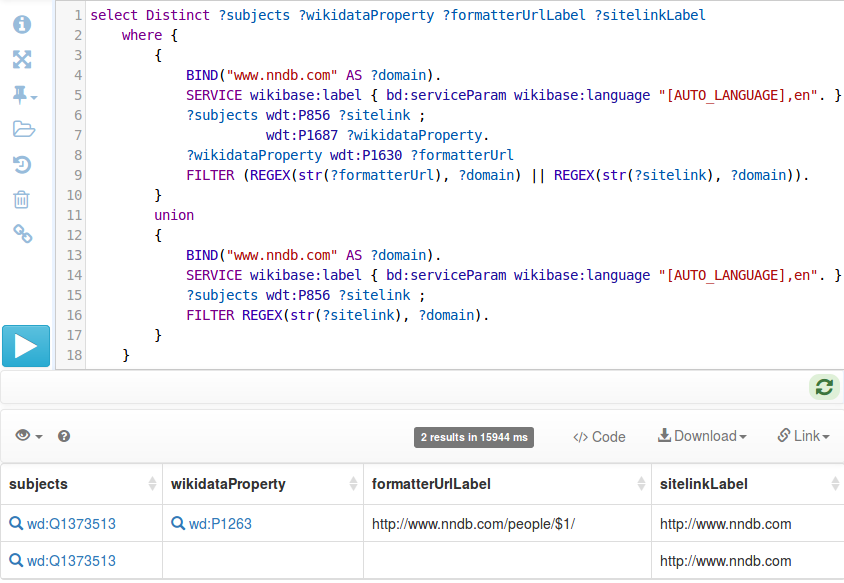
\includegraphics[width=\linewidth]{Sources/Img/c04_01.png}
    \captionof{figure}{Some here}
\end{center}

\section{Lo script}

\subsection{Struttura del progetto}
Il progetto presenta una cartella assets contenente tutti i file di input e output, i json di configurazione e i log degli errori; nella cartella business sono contenuti i servizi,
i metodi di utilità e le query. La cartella domain contiene i modelli e le localizations (nel file localizations.py sono definite anche una serie di costanti da settare a seconda 
delle esigenze per configurare lo script). 

In tests abbiamo tutte le classi di test basate sulla libreria unittest, come per il Client $C\#$ anche in questo caso è stato configurato Travis per far eseguire i test 
automaticamente ad ogni pull-request. Infine nella root del progetto abbiamo l'entry point dello script (main.py) e l'entry point dei test (test.py), i requirement per il package manager 
e il file di configurazione strephit.py nel caso si voglia lanciare lo script in un virtualenv tramite la libreria click.

\begin{lstlisting}[style=SPARQLStyle]
    select Distinct ?subjects ?wikidataProperty ?formatterUrlLabel ?sitelinkLabel
    where {
        {
            BIND("www.nndb.com" AS ?domain).
            SERVICE wikibase:label { bd:serviceParam wikibase:language "[AUTO_LANGUAGE],en". }
            ?subjects wdt:P856 ?sitelink ;
                      wdt:P1687 ?wikidataProperty.
            ?wikidataProperty wdt:P1630 ?formatterUrl
            FILTER (REGEX(str(?formatterUrl), ?domain) || REGEX(str(?sitelink), ?domain)).
        }
        union
        {
            BIND("www.nndb.com" AS ?domain).
            SERVICE wikibase:label { bd:serviceParam wikibase:language "[AUTO_LANGUAGE],en". }
            ?subjects wdt:P856 ?sitelink ;
            FILTER REGEX(str(?sitelink), ?domain).
        }
    }
\end{lstlisting}

\subsection{Algoritmo}
Istanziando l'oggetto QuickStatementsService vengono caricati automaticamente in memoria i mappings presenti nella cartella assets; 
i mappings sono dei file json di salvataggio in cui lo script salva i risultati delle le chiamate, all'end-point SPARQL, già effettuate.

\begin{lstlisting}[style=jsonStyle, caption=Some Code]
    "www.nndb.com": [
        {
            "db_id": "Q1373513", 
            "db_property": "S1263", 
            "to_upper_case": false, 
            "url_pattern": "http://www.nndb.com/people/$1/"
        }
    ], 
\end{lstlisting}

Il metodo \code{add\u db\u references\u async()} cicla su ogni riga del dataset e per ogniuna di esse chiama un handler (\code{add\u db\u references\u async\u handler()}), passandogli un oggetto 
QuickStatement contenente tutte le informazioni della riga, che procede con l'analisi della URL e la generazione dei riferimenti mancanti.

A questo punto, in modo sincrono o asincrono, a seconda del settaggio delle costanti in localizations.py (\code{IS\u ASYNC \u MODE = True/False}), 
viene chiamato il metodo \code{generate\u db\u reference()} che provvede a controllare che nei mappings ci sia già una entry con formatter URL compatibile 
con la URL del quickstatement e a generare i riferimenti mancanti.
Se nei mappings non esiste nessuna entry compatibile con la URL allora viene chiamato il metdo \code{new\u mapping()} che provvede a chiamare l'end-point SPARQL 
e a selezionare il risultato migliore per aggiungerlo ai mappings. 
Se la costante \code{MAP\u ALL\u RESPONSES} viene settata a \code{True}, ogni risposta del endpoint SPARQL viene salvata interamente nei mappings, questo previene qualsiasi altra chiamata all'endpoint 
per un determinato dominio ma accresce la dimensione dei mappings a dismisura e rende di conseguenza la ricerca più lenta.
 
\subsection{Refresh delle URL}
Nel dataset analizzato alcuni domini erano deprecati tant'è che tentando di accedervi da un browser si veniva reindirizzati ad altri domini oppure era avvenuto il passaggio da http ad https.

Per non perdere questi riferimenti si è deciso di implementare anche una funzionalità che data una lista di domini va a refreshare tutte le URL aventi tali domini e ad eliminare le 
righe contenenti URL inesistenti.

A fine procedura vengono salvati i log con la lista di url modificate e con la lista di righe eliminate dal dataset.


      \newpage     
      \chapter{Conclusioni}
Personalmente ritengo che l'esperienza di tesi sia stata molto positiva in quanto ho avuto la possibilità di entrare in contatto con diverse realtà lavorative fuori dal comune; 
sotto il profilo tecnico questo progetto mi ha portato ad apprendere molte nuove tecnologie che non conoscevo e a rafforzare conoscenze pregresse.

La prima parte, se pur non particolarmente complessa, è stata interessante perchè riguardava l'intero ciclo di vita di una libreria, dall'implementazione alla pubblicazione;
mi ha dato modo di rafforzare le nozioni di programmazione in C$\#$ e di seguire, per la prima volta, il deploy di una libreria su Nuget. 
La libreria è funzionante e ad oggi conta un centinaio di download, risultato sicuramente positivo.

La seconda parte si è rivelata, alla fine, un'analisi fine a se stessa, non si sono ottenuti risultati utili per poter ottimizzare l'algoritmo esistente;
nonostante ciò la ritengo personalmente un'esperienza positiva dato che mi ha permesso di provare svariate nuove tecnologie molto utili, prima fra tutte Docker. 

Mi ha colpito molto l'elevata complessità insita nel problema della valutazione prestazionale di un processo; 
infatti nel corso dell'analisi sono stati provati svariati javaagent, per monitorare il processo, che regolarmente risultavano inattendibili, 
in parte per l'interazione con altri processi e in parte per il ridotto scope di visibilità del software di monitoraggio stesso 
(senza contare la presenza di svariati fattori aleatori come l'azione del Garbage Collector).

Altra cosa che mi ha sorpreso molto è stato l'incredibile calo prestazionale della funzione hash all'aumentare delle dimensioni del dominio, tanto che la computazione dell'hash stesso 
richiedeva più tempo della ricerca binaria.

Penso sia comunque possibile trovare un'implementazione migliore dell'attuale; sarebbe un interessante spunto di ricerca ulteriore valutare se sia possibile creare una 
funzione hash ad hoc per questo problema; sarebbe anche interessante valutare implementazioni basate su strutture dati salvate su disco anzichè in memoria 
(database, indici di Lucene\cite{lucene}, ecc.), anche se sicuramente i tempi di risposta aumenterebbero di qualche ordine di grandezza per il solo accesso al disco. 

La terza parte mi ha permesso di conoscere il mondo di Wikidata e del semantic web più in generale, dandomi l'opportunità di contribuire, per la prima volta, 
ad un progetto open source così rilevante.

Si è ottenuto il risultato sperato, in quanto lo script funziona correttamente, tuttavia sarebbe interessante riuscire ad ottimizzare lo script visto che attualmente, 
per computare un dataset da 500.000 righe, impiega qualche ora; 
va da sè che spesso si hanno ritardi, anche di svariati secondi, totalmente indipendenti dallo script (connessione ad internet, tempo di attesa per le query SPARQL 
e per il "refresh" delle URL deprecate, tramite chiamate HTTP); tolti questi punti sicuramente si possono ottimizzare le routine maggiormente usate nello script 
per abbassare i tempi di computazione.

In conclusione voglio ringraziare tutti coloro che mi hanno aiutato e seguito in questo progetto di tesi.
      \newpage     
    \endgroup

    % bibliografia in formato bibtex
    
    \addcontentsline{toc}{chapter}{Bibliografia} % aggiunta del capitolo nell'indice
    \bibliographystyle{plain} % stile con ordinamento alfabetico in funzione degli autori
    \bibliography{biblio}
    %% Nella bibliografia devo avere tutte le fonti consultate; va redatta in ordine alfabetico sul cognome del primo autore. 
    %% LIBRI
    %% Cognome e iniziale del nome autore, la data di edizione, titolo, casa editrice, eventuale numero dell’edizione. 
    %% SITOGRAFIA
    %% Lista di indirizzi Web disposti in ordine alfabetico. 
    %% URL, cognome e nome dell’autore, il titolo, sottotitolo, data di ultima consultazione della risorsa (gg/mm/aaaa).
    \titleformat{\chapter}
        {\normalfont\Huge\bfseries}{Allegato \thechapter}{1em}{}
    % sezione Allegati - opzionale
    \appendix
    % \chapter{Titolo primo allegato}

% Lorem ipsum dolor sit amet, consectetur adipiscing elit. Donec sed nunc orci. Aliquam nec nisl vitae sapien pulvinar dictum quis non urna. Suspendisse at dui a erat aliquam vestibulum. Quisque ultrices pellentesque pellentesque. Pellentesque egestas quam sed blandit tempus. Sed congue nec risus posuere euismod. Maecenas ut lacus id mauris sagittis egestas a eu dui. Class aptent taciti sociosqu ad litora torquent per conubia nostra, per inceptos himenaeos. Pellentesque at ultrices tellus. Ut eu purus eget sem iaculis ultricies sed non lorem. Curabitur gravida dui eget ex vestibulum venenatis. Phasellus gravida tellus velit, non eleifend justo lobortis eget. 

% \section{Titolo}
% Lorem ipsum dolor sit amet, consectetur adipiscing elit. Donec sed nunc orci. Aliquam nec nisl vitae sapien pulvinar dictum quis non urna. Suspendisse at dui a erat aliquam vestibulum. Quisque ultrices pellentesque pellentesque. Pellentesque egestas quam sed blandit tempus. Sed congue nec risus posuere euismod. Maecenas ut lacus id mauris sagittis egestas a eu dui. Class aptent taciti sociosqu ad litora torquent per conubia nostra, per inceptos himenaeos. Pellentesque at ultrices tellus. Ut eu purus eget sem iaculis ultricies sed non lorem. Curabitur gravida dui eget ex vestibulum venenatis. Phasellus gravida tellus velit, non eleifend justo lobortis eget. 

% \subsection{Sottotitolo}
% Lorem ipsum dolor sit amet, consectetur adipiscing elit. Donec sed nunc orci. Aliquam nec nisl vitae sapien pulvinar dictum quis non urna. Suspendisse at dui a erat aliquam vestibulum. Quisque ultrices pellentesque pellentesque. Pellentesque egestas quam sed blandit tempus. Sed congue nec risus posuere euismod. Maecenas ut lacus id mauris sagittis egestas a eu dui. Class aptent taciti sociosqu ad litora torquent per conubia nostra, per inceptos himenaeos. Pellentesque at ultrices tellus. Ut eu purus eget sem iaculis ultricies sed non lorem. Curabitur gravida dui eget ex vestibulum venenatis. Phasellus gravida tellus velit, non eleifend justo lobortis eget. 


% \chapter{Titolo secondo allegato}

% Lorem ipsum dolor sit amet, consectetur adipiscing elit. Donec sed nunc orci. Aliquam nec nisl vitae sapien pulvinar dictum quis non urna. Suspendisse at dui a erat aliquam vestibulum. Quisque ultrices pellentesque pellentesque. Pellentesque egestas quam sed blandit tempus. Sed congue nec risus posuere euismod. Maecenas ut lacus id mauris sagittis egestas a eu dui. Class aptent taciti sociosqu ad litora torquent per conubia nostra, per inceptos himenaeos. Pellentesque at ultrices tellus. Ut eu purus eget sem iaculis ultricies sed non lorem. Curabitur gravida dui eget ex vestibulum venenatis. Phasellus gravida tellus velit, non eleifend justo lobortis eget. 

% \section{Titolo}
% Lorem ipsum dolor sit amet, consectetur adipiscing elit. Donec sed nunc orci. Aliquam nec nisl vitae sapien pulvinar dictum quis non urna. Suspendisse at dui a erat aliquam vestibulum. Quisque ultrices pellentesque pellentesque. Pellentesque egestas quam sed blandit tempus. Sed congue nec risus posuere euismod. Maecenas ut lacus id mauris sagittis egestas a eu dui. Class aptent taciti sociosqu ad litora torquent per conubia nostra, per inceptos himenaeos. Pellentesque at ultrices tellus. Ut eu purus eget sem iaculis ultricies sed non lorem. Curabitur gravida dui eget ex vestibulum venenatis. Phasellus gravida tellus velit, non eleifend justo lobortis eget. 

% \subsection{Sottotitolo}
% Lorem ipsum dolor sit amet, consectetur adipiscing elit. Donec sed nunc orci. Aliquam nec nisl vitae sapien pulvinar dictum quis non urna. Suspendisse at dui a erat aliquam vestibulum. Quisque ultrices pellentesque pellentesque. Pellentesque egestas quam sed blandit tempus. Sed congue nec risus posuere euismod. Maecenas ut lacus id mauris sagittis egestas a eu dui. Class aptent taciti sociosqu ad litora torquent per conubia nostra, per inceptos himenaeos. Pellentesque at ultrices tellus. Ut eu purus eget sem iaculis ultricies sed non lorem. Curabitur gravida dui eget ex vestibulum venenatis. Phasellus gravida tellus velit, non eleifend justo lobortis eget. 



\end{document}
